\section{Database}

\subsection{Modello E/R}%
\label{sec:modelloer}

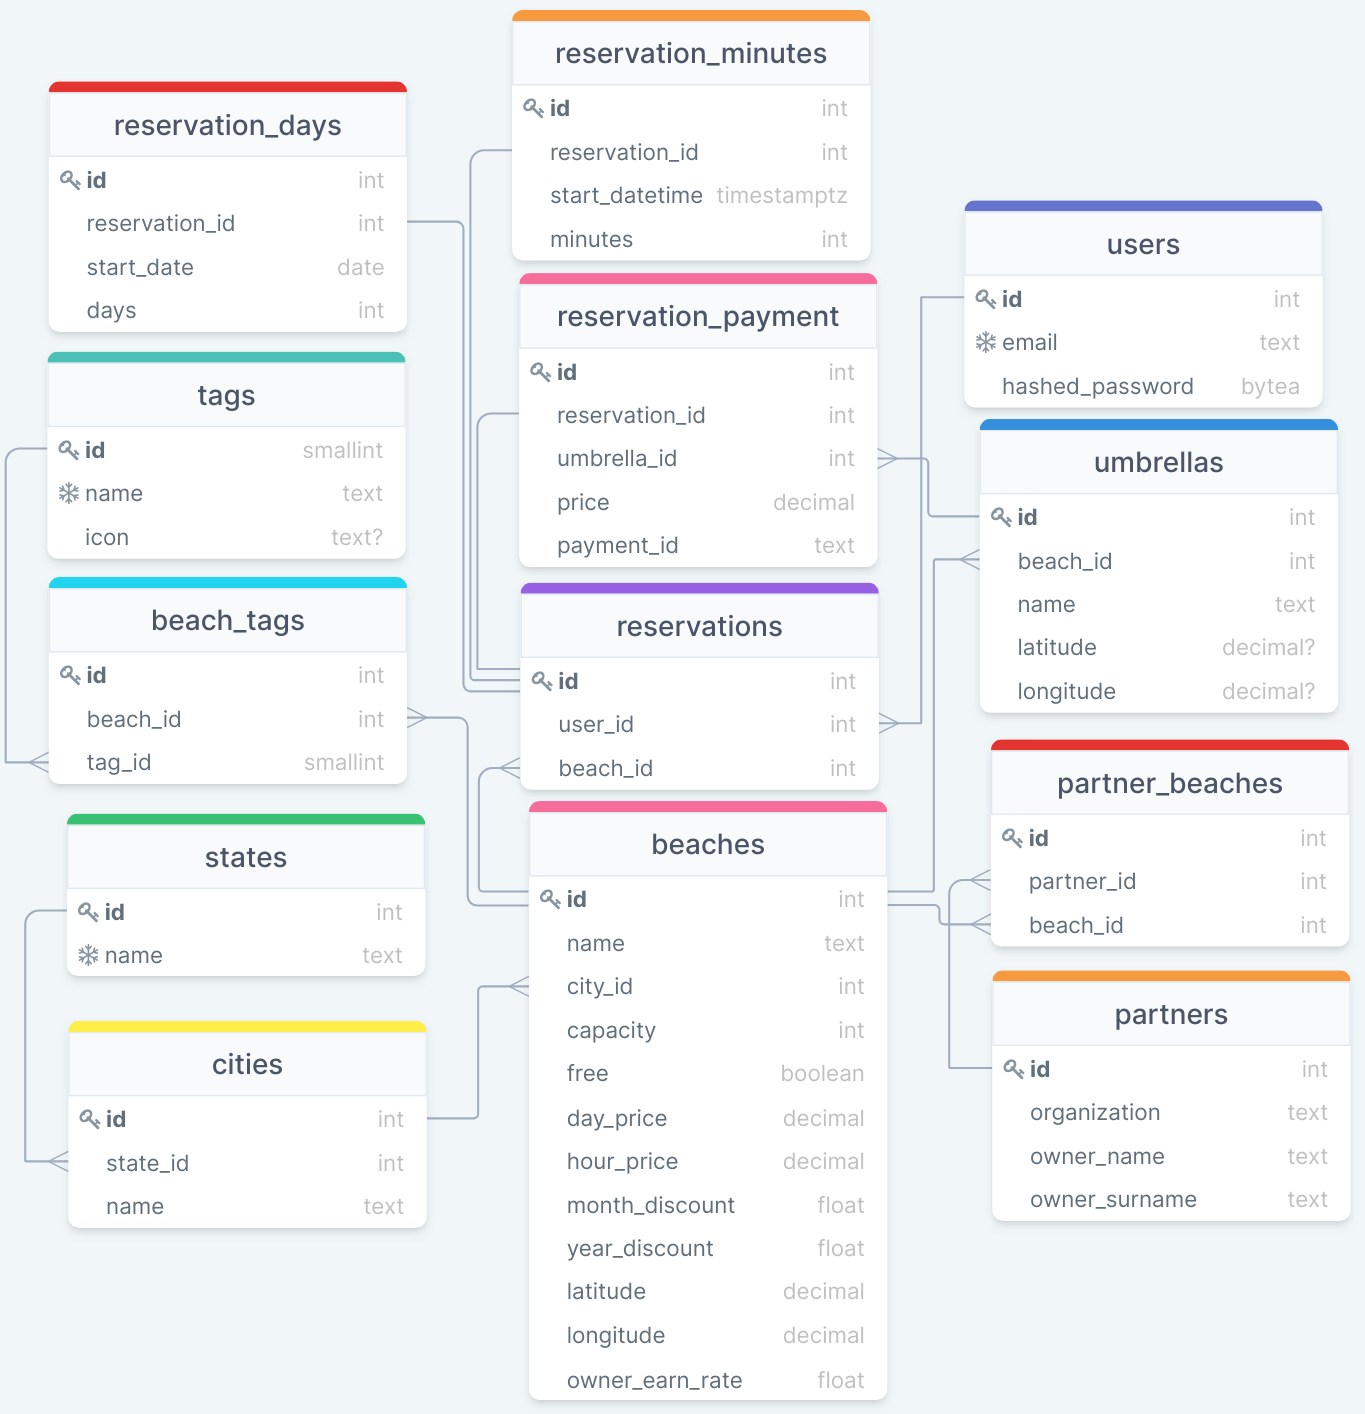
\includegraphics[width=\linewidth]{modelloer.png}

Le tabelle reservation\_days, reservation\_minutes e reservation\_payment sono tabelle in relazione uno ad uno con la tabella reservations. Queste aggiungono informazioni situazionali alla prenotazione.

\begin{itemize}
    \item \textbf{reservation\_days}: Aggiunge informazioni sulla prenotazione se la prenotazione \`e della durata di giornate intere. (una o pi\`u)
    \item \textbf{reservation\_minutes}: Aggiunge informazioni sulla prenotazione se la prenotazione \`e della durata di alcuni minuti o ore.
    \item \textbf{reservation\_payment}: Aggiunge informazioni sulla prenotazione di \allowbreak{ombrelloni}. Non \`e presente se viene prenotata una spiaggia libera. Contine informazioni sulla transazione PayPal.
\end{itemize}

Le informazioni per il pagamento degli Stabilimenti Partner non sono incluse all'interno della tabella partners siccome sono dati sensibili. I dati sensibili insieme al \emph{salt} delle password devono essere salvati in un database separato per permettere un livello di sicurezza superiore.

Gli ID di tutte le tabelle sono autogenerate con le sequenze di Postgres. Quando vengono definite le tabelle viene utilizzato il tipo ``serial'' e le sue varianti, ``smallserial'' e ``bigserial'' che corrispondono rispettivamente ai tipi ``int'', ``smallint'' e ``bigint'' ma insieme ad essi vengono creati degli oggetti speciali chiamati sequenze. Le sequenze permettono di tenere traccia dell'ultimo ID inserito e scelgono in automatico il prossimo quando viene inserito un nuovo record all'interno della tabella.
